\section{Karotz}
Karotz.com (2012)\cite{karotz} describes Karotz as a robot shaped 
as a bunny that can interact with
a user through light, ear movement and sound. It can also take
input through a button, moving its ears, an RFID (Radio-frequency identification) chip, voice
commands and serial (Internet) communication.

The project includes developing an application for the Karotz
platform that will serve as an addition to the mobile applications.
It is therefore necessary to study its interfaces, development
methods and API of the machine.

\begin{figure}[h]
	\centering
		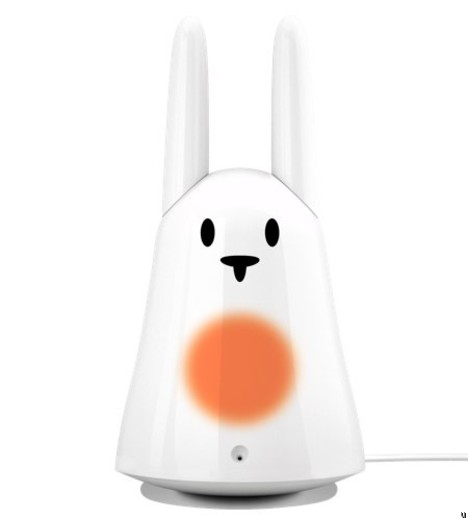
\includegraphics[height=10cm]{Pictures/karotzimg}
	\caption{Karotz: A bunny-shaped robot}
	\label{fig:karotz}
\end{figure}

\subsection{Application Platform}
Karotz application (called ``Appz'') are installed through an
online platform located on the Karotz web site. They can be
launched on the Karotz itself either through a scheduler, voice
commands or an RFID chip. These RFID chips come in various shapes,
sizes and colors. Figure \ref{fig:flatnanoz} and Figure 
\ref{fig:nanoztag} show examples of the different kinds of ``nanoz'',
that are small figures with an integrated RFID chip.

\begin{figure}
	\begin{minipage}[b]{0.4\linewidth}
		\centering
			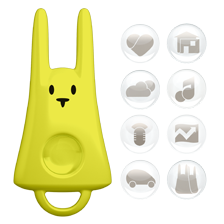
\includegraphics[width=0.30\paperwidth]{Pictures/FlatnanozYellow}
		\caption[Flatnanoz]{A flat nanoz--flatnanoz-- a figure with an RFID chip used to provide input to a Karotz.}
		\label{fig:flatnanoz}
	\end{minipage}
	\hspace{3cm}
	\begin{minipage}[b]{0.4\linewidth}
		\centering
			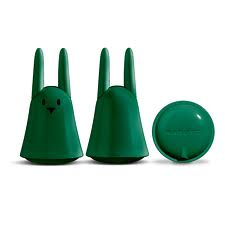
\includegraphics[width=0.30\paperwidth]{Pictures/NanoztagGreen}
		\caption[Nanoztag]{A round nanoz--nanoztag-- a figure with an RFID chip used to provide input to a Karotz.}
		\label{fig:nanoztag}
	\end{minipage}
\end{figure}

Some mentionable applications made by other developers are 
``At Home'', an application that may register that someone checks 
in at the Karotz, and send an e-mail to a predetermined mail 
address, so children may tell their parents that they are home. 
``Twitter for Karotz'' may read you tweets and post tweets based 
on voice-commands. Another mention is ``Weather'' which may tell 
you the forecast for the day or the following day. It seems all 
applications registered at the Karotz website are fairly simple 
and have little functionality.

As for launching the BLOPP application, the times for the scheduler must
be manually set through the Karotz web site, so it cannot be 
used for notifications directly. The best option for the BLOPP 
implementation would therefore be to set a scheduler to start
every day at 00:00 and stop every day at 23:59. This way it can
be ensured that the application is always running, updating
itself with medications, status and times, and a timer can be
used to schedule notifications.

%\subsection{The two APIs}
The Karotz can be programmed in two different ways: either
through a web REST (Representational State Transfe) framework, 
or with JavaScript that runs as an embedded program on the robot itself.

The requirement that a REST program would have to be hosted
somewhere, combined with the fact that an embedded program 
provides more flexibility in terms of local storage to limit the
amount of information sent over a network makes the JavaScript
framework a more suitable choice for the BLOPP project.

%\subsection{Karotz Output Channels}
The Karotz has a few ways of providing output to the end-user. It
can be asked to
\begin{itemize}
    \item play sound files;
    \item move its ears;
    \item speak, using a TTS (text-to-speach) engine;
    \item illuminate its stomach in different colors;
    and
    \item communicate over the internet with HTTP (Hyper Text Transfer Protocol) GET and POST 
          methods.
\end{itemize}

For providing user commands, TTS could be an option if the engine
supported Norwegian, but since the language options are limited to
English, French, German and Spanish, speech will have to be
created by recording sound files and playing them with the
multimedia engine.